
\section{Entwicklung einer Handlungsempfehlung}
\label{sec:Handlungsempfehlung}
In einem wettbewerbsintensiven Umfeld reicht es häufig nicht aus die Bedürfnisse der Anwender zu verstehen und innovative IT-Services zu implementieren. Stattdessen ist die schnelle Reaktionsfähigkeit und das zeitnahe Bereitstellen gegenüber Konkurrenzunternehmen von erheblicherer Bedeutung. Infolgedessen etablieren 62 Prozent aller Unternehmensentwickler CI/CD-Tools innerhalb ihrer Bereitstlelungsprozesse. Die kontinuierliche Integration und Bereitstellung von Software bietet dabei insbesondere für CEs erhebliche Vorteile. Obwohl einzelne Module einer CEA grundsätzlich isoliert voneinadner betrieben werden, können Abhängigkeiten zwischen diesen entsehen. Im Kontext eines Composable-ERP-Systems könnte es etwa erforderlich sein, dass die in dem Vertriebsmodul abgewickelt Verkäufe in das Finanzwesen übertragen werden müssen. Insbesondere bei der Zusammenarbeit vieler Entwickler, kann diese Integration zu erheblichem Koodinationsaufwand führen. Wenn Teams nicht in der Lage sind effektiv miteinander zu kommunizieren, besteht das Risiko, dass im Zusammenspiels einzelner Komponenten Fehler entstehen. Um dieser Herausforderung zu begegnen, bietet sich die Implementierung einer CI/CD-Pipeline. Dabei wird der lokale Quell-Code der Etnwickler kontunierlich und automatisiert mit dem Hauptzweige des Repositories zusammengeführt und mit dem bestehenden Code getestet. Statt Code-Reviews und Validierungen erst in einer späten Phase des Softwareerstellungszykluses abzuwickeln (\textit{Shift-Right}), werden Tests bereits während der Entwicklung durchgeführt (\textit{Shift-Left}). Nach Erstellung einer Funktionalität bekommen Entwickler über verschiedene Kommunikationskanaläle (z.B. E-Mail) somit unmittelbares Feedback und können den Service optimieren, bis dieser den Produktstandards des Unternehmens entspricht. Dieser Ansatz zielt darauf ab, eine frühzeitige Identifikation und Behebung von Fehlern zu erleichtern. Darüber hinaus ermöglichen CI/CD-Pipelines einen Aufbau standardisierter Testumgebungen. Damit können neue Features in Systemumgebungen getestet werden, bei welchen Betriebssystem, Systembibliothenek, Abhängigkeiten und Konfigurationseinstellungen an die Produktionsumgebung angepasst sind. Somit entfällt ein manuelles Aufsetzen der Testinfrastruktur, wodruch CEs ihre Ressourcen vermehrt auf das Kerngeschäft, also die Entwicklung neuer ERP-Funktionalitäten, konzentrieren können. Ein zentrales Monitoring aller CI/CD-Pipelines einer CEA, können dazu beitragen, die Code-Qualität zu überwachen und kontinuierlich zu verbessern. Die Dasboads der CI/CD-Tools unterstützen bei der Visaulisierung verschiedener Metriken des Bereitstellungsprozesses. So können etwa Perfomance-Validierungen, welchen das Testen einzelner Funktionalitäten unter verschiedenen Lastbedingungen automatisieren, analysiert werden. Diese Metriken können anschließend in einen historischen Datenkontext eingeordnet werden, womit Entwickler-Teams Trends in der Code-Qualität identifizieren können. Der von Panorama Consultings Solutions veröffentlichte ERP Report 2019 zeigt, dass ERP-Systeme aufgrund der Geschwindigkeit mit welcher sich Unternehmenstechnologien und Marktdynamiken entwickeln, zukunftsorientiert sein müssen. Dies bedarf einer kontinuierlichen Aktualisierung um moderne Funktionen, ohne dabei auf wiederholte kostspielige Upgrades zurückgreifen zu müssen. Dafür ist es von essenzieller Bedeutung, dass nicht nur das Testen, sondern ebenfalls die Bereitstellung kontinuierlich und automatisiert durchgeführt wird. Das unmittelbare Kompilieren, Validieren und Versionieren bei einer Integration, ermöglicht ein mehrfaches tägliches Ausrollen von neuen Anwendungsverisonen. Dies führt zur Verkürzung des Time-To-Values, dem Intervall bis die von dem Softwareunternehmen entwickelte Lösung ersten Kundennutzen herbeiführt. Durch die Zerlegung großer Epics in kleine kontinuierliche Feature-Releases besteht zwar die Möglchkeit, dass der Kundennutzen im Vergleich zur vollständigen Einführung abgeschwächt wird, jedoch ermöglicht eine solche Früheinführung Vorsprung gegenüber Konkurrenten. Damit können Unternehmen bereits frühzeitig Rückmeldung von Anwendern erhalten, welches im Anschluss schnell verarbeitet werden kann \cite[9]{Halstenberg.2020}. Dieser inkrementelle Ansatz führt dazu, dass Entwickler und Betriebsteams einen beschleunigten Lernprozess durchlaufen und ihre Arbeitsweise entsprechend anpassen können. Tortz erfolgreicher Abwicklung aller Validierungen, besteht die Möglchkeit, dass fehlerhafter Code von dem CI/CD-Prozess auf die Produktionssysteme geladen wird. Die Verwendung kleiner Code-Bereitstellungszyklen erleichtert Entwickler jedoch die Identifikation von Problemen und ermöglicht somit eine zügige Fehlerbehebung. Eine korrespondierende Erkenntnis geht ebenfalls aus dem State of CD Report 2022 hervor. So soll eine schnelle Bereitstellung, ebenfalls eine zügigere Behebung von Fehlern (s. Tab. \ref{tab:Error}). 
\begin{center}
	\begin{table}[H]
		\centering
		\scalebox{0.5}{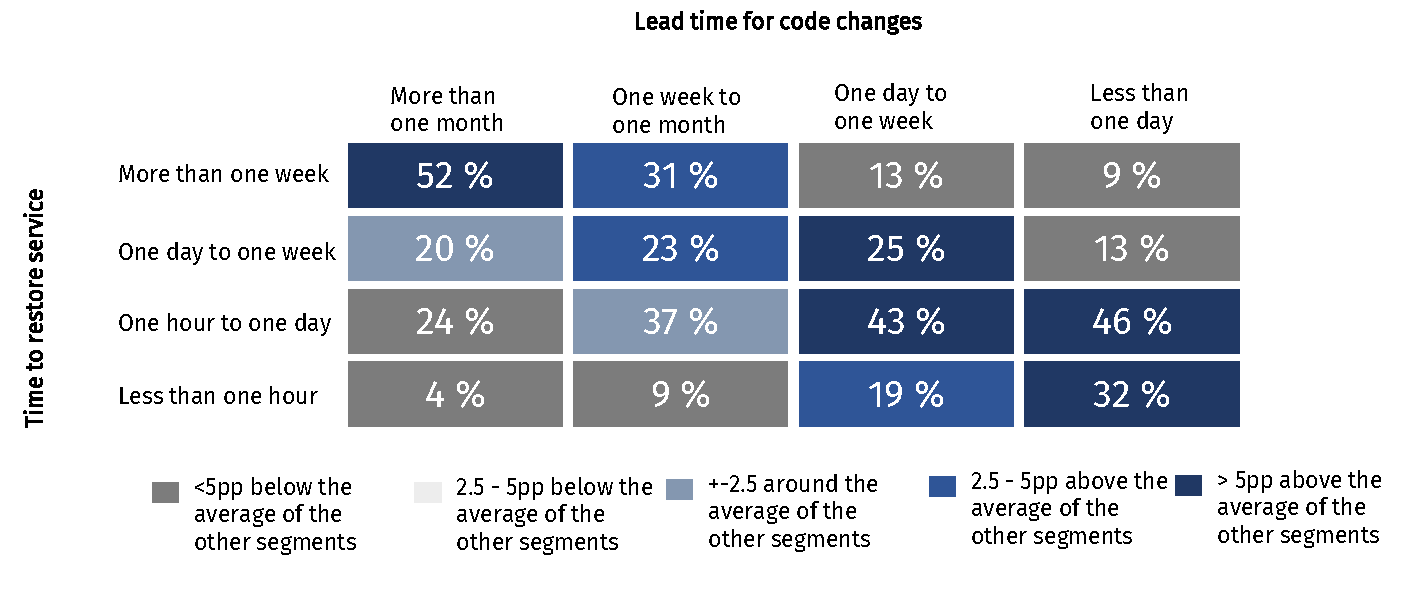
\includegraphics{Error}}
		\caption[Korrelation zwischen Vorlaufzeit und Fehlerate bei der Bereitstellung]{Korrelation zwischen Vorlaufzeit und Fehlerrate bei der Bereitstellung. In Anlehnung an Berry.}
		\label{tab:Error}
	\end{table}
\end{center}
\vspace*{-15mm} 
Entschließt sich ein CE Bereistellungsprozesse zu automatisieren, sollte dieses dabei strategisch vorgehen. So empfiehlt Experte 5, Software-Architekt des SAP DTS, ein schrittweises Implementieren der Pipeline. Dabei sollte ein Entwicklungsteam zunächst Erfahrung mit der Automatisierung einfacher isolierter Prozesse sammeln \cite[Z. 8 ff.]{SoftwareArchitektSAPDTSIntegration.}. Anschließend kann ein Unternhemen alle verbleibenden Schritte, welche zur Bereitstellung benötigt werden, in einem kontrollierten Tempo automatiseren. Bei der Einführung von CI/CD ist es ebenso entscheident, dass Unternehmen spezifische Anforderungen abdeckende Tools verwenden. Dafür wurde im Rahmen dieser Arbeit ein Entscheidungs-Framework entworfen. Mit diesem wurde evaluiert, welches Pipeline-Tool zur Automatisierung der CI/CD-Prozesse für CEA den größten Mehrwert birgt. Unter Berücksichtigung der in Kapitel \ref{sec:Bewertung} abgewickelten Analyse, kann Azure Pipelines als das optimale CI/CD-Tool angesehen werden. Aus diesem Kontext lassen sich für das Pipeline-Tool Vorteile ableiten. Azure Pipelines unterstützt die Programmbibliothek Project Piper, mit welcher essenzielle Schritte für das Bauen, Testen und Bereitstellen von SAP-CAP-Node- und SAP-UI5-Anwendungen, ausgeliefert werden. Die Bereitstellung vorimplementierter Schritte stellt sicher, dass sämtliche Compliance-Standards der SAP, wie Sicherheits- und Datenschutzbestimmungen, Branchenvorschriften oder interne Richtlinien, eingehalten werden. Obwohl die vorliegende Arbeit zur Beratung externer Kunden konzipiert ist, welche nicht verpflichtet sind, diese Richtlinien einzuhalten, sind diese oft in kritischen Sektoren, wie der Finanz- oder Versicherungsindustrie, tätig, bei welchen ebenfalls strikte Regularien gelten. Durch die Bereitstellung dieser standardisierten Bibliothek entfällt für die Entwickler somit die Notwendigkeit einer zeitaufwändigen Implementierung dieser Schritte. Daneben, dass CEs auf diese Weise in der Lage sind, neue Services schnell bereitzustellen, erleichtert eine zentrale Bibliothek ebenfalls Aktualisierung und Pflege einzelner Pipeline-Schritte. Des Weiteren werden durch die Programmbibliothek Project Piper ebenfalls umfassende Bereitstellungsfunktionalitäten zur Verfügung gestellt. So umfasst diese neben vorimplementierten Schritten zum Ausrollen von Anwendungen auf der SAP BTP, ebenfalls ein Blue/Green-Deployment. Das Blue-Green-Deployment stellt eine effektive Möglichkeit dar, Software unter Produktionsbediungen zu testen und kritische Ausfallszeiten bei der Bereitstellung von Software zu vermeiden. Dies spielt insbesondere dann eine wichtige Rolle, wenn Fehler in einem Microservice eines ERP-Systems auftreten, jedoch das herkömmliche Bereitstellen einer neuen Anwendungsversion aufgrund der durch die Initalisierung bedingten Ausfallzeit, zu unflexibel ist. Ein weiteres von CEs verwendetes Bereitstellungskonzept ist das Multi-Cloud-Deployment. Damit können einzelne Module, wie CRM- oder SCM-Komponenten, auf unterschiedlichen Cloud-Plattformen betrieben werden. Neben einer Bereitstellung auf etablierten Cloud-Plattformen wie Google-Cloud oder Amazon Web Services ermöglicht Azure Pipelines ebenfalls eine nahtlose Integration mit den eigenen Cloud-Diensten. Dieser Integrationsvorteil erstreckt sich ebenfalls auf andere Services, welche innerhalb des Azure-Ökosystems bereitgestellt werden. So umfasst dieses darüber hinaus Dienste, wie eine Entwicklungsumgebung, ein Projektmanagement- und Monitoring-Tool sowie ein Artefakt-Repository, welche mit geringem Aufwand in die CI/CD-Pipeline integriert werden können. Laut Experte 5, Software-Architekt des SAP DTS, stellt Technologieoffenheit einen wichtigen Aspekt für CEs dar \cite[Z. 8 ff.]{SoftwareArchitektSAPDTSIntegration.}. Obwohl die Evaluation dieser Arbeit auf SAP-Technologien beschränkt ist, besteht die Möglichkeit, dass sich ein CEs dazu entscheidet einzelne Services auf anderen Technologien aufzubauen. Azure Pipelines stellt im Standard bereits unzählige Build-Tools sowie Test-Frameworks zur Verfügung. Sollte dieser jedoch nicht ausreichend sein, können mit Azure Pipelines ebenfalls Docker-Container aufgebaut werden. Mit diesen besteht Möglichkeiten Abhängigkeiten, wie Software-Treiber, in einem Container zu installieren, ohne von der Laufzeitumgebung der Pipeline abhängig zu sein. Azure Pipelines kann darüber hinaus zur Vereinfachung des Entwicklungsprozesses beitragen. So ist es  Entwickler möglich, Test der Integration-Pipeline unmittelbar aus der Visual-Studio-Code-Umgebung auszuführen ohne, dass Features zunächst in das Repository geladen werden müssen. Des Weiteren können mit dem CI/CD-Tool Pipeline-Implementationen sowohl lokal aus den Entwicklungsumgebungen, als auch zentral in dem Azure-Dashboard bearbeitet werden. Diese Praktikabilität ergibt sich ebenfalls bei der Ausführung der CI/CD-Pipelines. Im Falle von Fehlschlägen einzelner Schritte, besteht die Möglichkeit, dass nur die fehlerhafte Schritte erneut ausgeführt werden. Auf diese Weise lassen sich bei temporären Problemen oder externen Abhängigkeiten, wie Ausfällen von Drittanbietern, Zeit und Rechenresourcen einsparen. Laut Experte 3 spielt dies insbesondere bei der Bereitstellung umfangreicher ERP-Services eine wichtige Rolle, da Pipeline-Schritte wie Code-Analysen mit unter über fünf Stunden in Anspruch nehemen können. Dies erwies sich ebenfalls im One-Strike Programm als einen bedeutenden Aspekt. In diesem Zusammenhang hat die SAP Maßnahmen ergriffen, um die Anzahl der Cloud-Provider, von welchen Dienste bezogen werden, zu reduzieren. Im Rahmen dieser Konsolidierung wurden Frontend-End-Pipelines für das S/4HANA-Core, welche zuvor auf Jenkins gehostet wurden, zu Azure migriert. Ein weiterer wesentlicher Aspekt für diesen Wechsel, waren Kostenüberlegungen. Durch die Nutzung einer SaaS-basierten CI/CD-Lösung können erhebliche Einsparchungen bei Aufwandspositionen, Hardwareinvestitionen oder Wartungs- und Support-Kosten erzielt werden. Dieser Aspekt birgt insbesondere für einen erheblichen Mehrwert für die CEA. Da Unternehmen mit dieser Architektur bestrebt sind, schnell auf distruptive Marktveränderungen zu reagieren, müssen diese in der Lage sein, Services wie CI/CD-Pipelines schnell auf- und abbauen bzw. skalieren können. Während in einem On-Premise-Modell hierfür ggf. hohe Investitionen erfoderlich sind, wird bei Azure in Abhängigkeit der Nutzung bezahlt (\textit{Pay-as-you-go}). Da die Bereitstellung von Services zum Kerngeschäft von Microsoft gehört, wird kontinuierlich in die Aktualisierung und Verbesserung der Azure-Infrastruktur investiert. Neben der Verwendung neuester Hardware wird die hohe Leistungsfähigkeit von Azure Pipelines ebenfalls durch das Bereitstellen von Optimierungsmechanismen sichergestellt. Dazu gehört etwa das parallele Ausführen verschiedener Pipeline-Schritte was insbesondere umfangreiche Testvorgängen Mehgrwert birgt. Ferner besteht die Möglichkeit der Verwedung von Caching-Mechanismen. Damit können Ressourcen, wie Artefakte oder Daten, welche während des Pipeline-Prozesses heruntergeladen werden, für weitere CI/CD-Workflows  auf der Cloud zwischengespeichert werden. Laut Experte 4, haben diese Konzepte dazu beitragen, dass der CI/CD-Prozess der internen Standardentwicklung um 35 Prozent beschleunigt wurde \cite[Z. 58 ff.]{TestDeveloperSAPHyperspaceAdoption&Onboarding.}. Obwohl Azure Pipelines die für eine CEA essenziellen Funktionalitäten bereitstellt, besteht die Möglichkeit, dass Unternehmen aufgrund situativer Gegebenheiten, Jenkins oder SAP CI/CD verwenden. Dafür ausschlaggebende Gründe werden in dem in Abb. \ref{fig:Entscheidungsbaum} dargestellten Entscheidungsbaum aufgeführt.
 \begin{center}
	\begin{table}[H]
		\centering
		\scalebox{0.5}{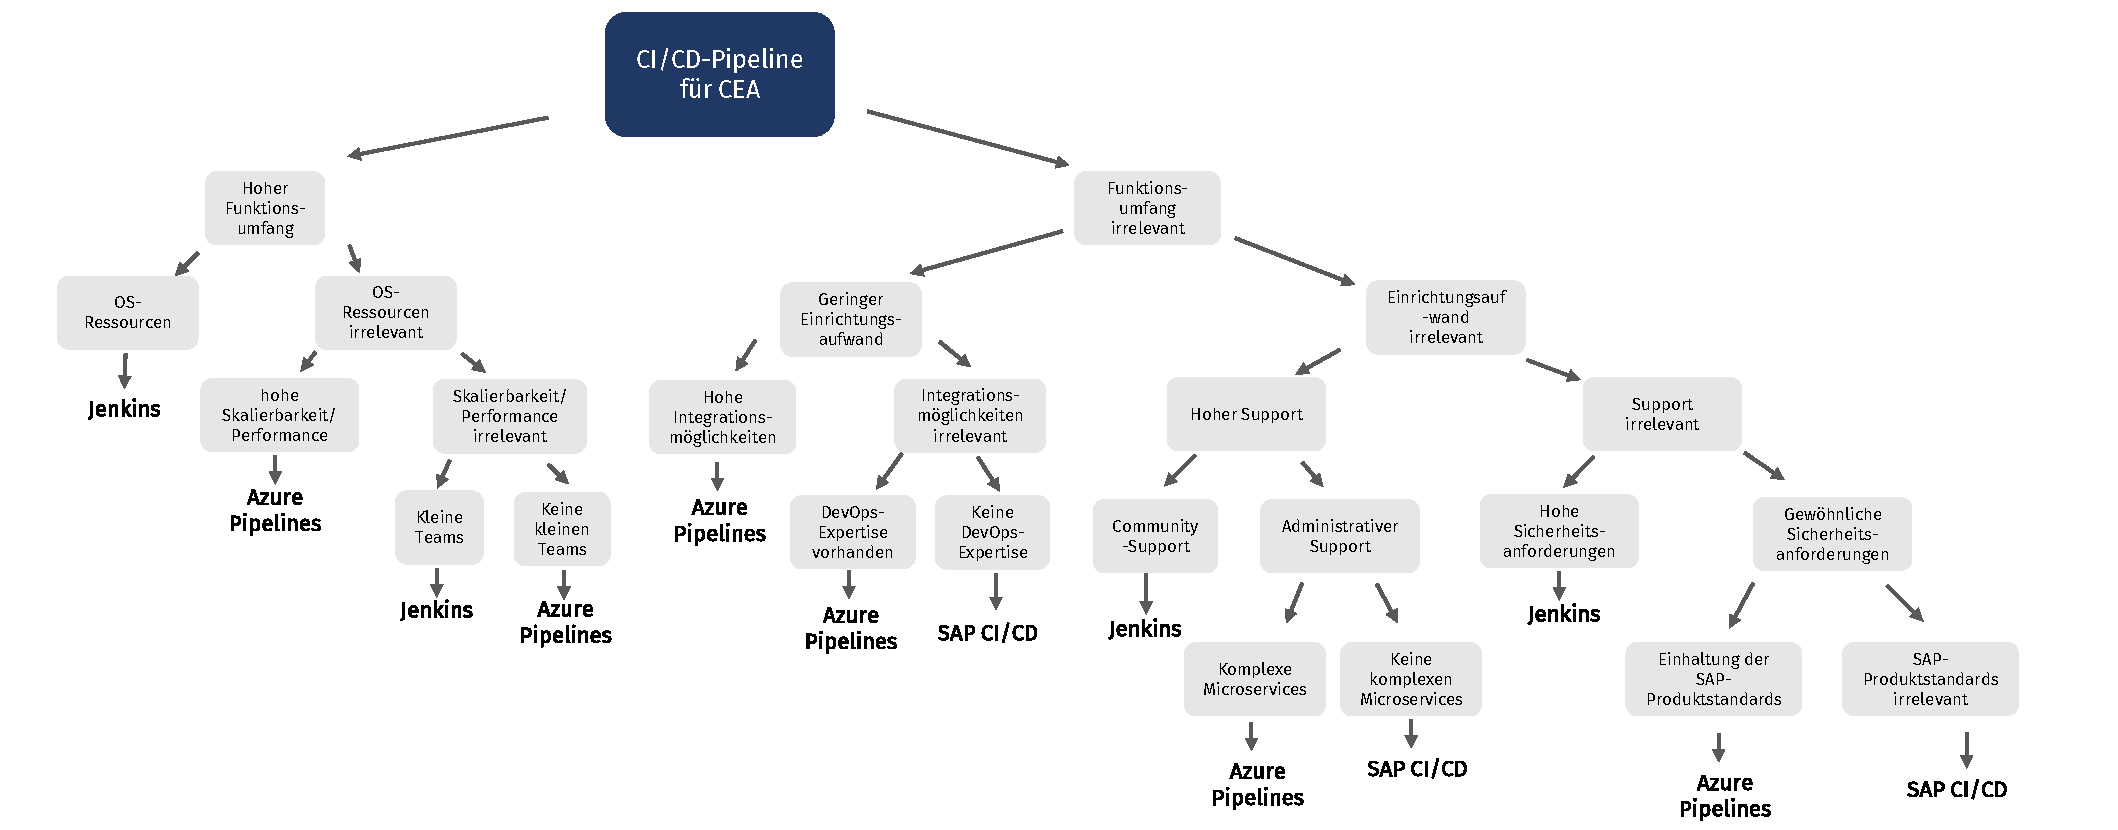
\includegraphics{Entscheidungsbaum}}
		\caption[Entscheidungsbaum für die Wahl eines CI/CD-Pipeline-Tools]{Entscheidungsbaum für die Wahl eines CI/CD-Pipeline-Tools. Eigene Darstellung.}
		\label{fig:Entscheidungsbaum}
	\end{table}
\end{center}
\vspace*{-15mm}
Laut Experte 1 sollte SAP CI/CD insbesondere von Kunden verwendet werden, welche nur über wenige Microservices verfügen und somit keine komplexen Anforderungen an den Bereitstellungsprozessen besitzen \cite[Z. 58 ff.]{ProductOwnerSAPBTPProd&Infra.}. Auch wenn mit SAP CI/CD für SAP CAP Node sowie SAP UI5 essenzielle Pipeline-Schritte bereitgestellt werden, verfügen Unternehmen mit diesem Tool in ihren Funktionalitäten eingeschränkt. Dies ist maßgeblich darauf zurückzuführen, dass das CI/CD-Tool ausschließlich eine Konfigurierung und keine Implementierung der Pipelines bereitstellt. Laut Experte 1 ist dieses Tool jedoch insbesondere für Kunden vorhergesehen, welche aus der traditionellen On-Premise-Umgebung auf die SAP BTP umsteigen \cite[Z. 58 ff.]{ProductOwnerSAPBTPProd&Infra.}. Hierbei besitzen Entwicklungs-Teams i.d.R. nicht über erforderliche DevOps-Kenntnisse, da diese zunächst mit dem Lernen allgemeiner Cloud-Konzepte, wie z.B. Programmier-Frameworks, beschäftigt sind. So soll das im Jahr 2020 veröffentlichte Tool kontinuierlich erweitert werden, um den wachsenden Anforderungen der Nutzer gerecht zu werden. Weiterhin empfiehlt sich dieses Tool für CEs, welche bereits ein umfangreiches Produktfolio der SAP besitzt und auch zukünftig auf SAP-Technologien setzen möchte. Eine weitaus höhere Flexibilität ergibt sich durch die Verwendung von Jenkins. Da dieses CI/CD-Tool On-Premise bereitgestellt wird, besitzt ein Unternehmen volle Kontrolle über die Gestaltung der Pipelines und kann diese somit auf die Bedürfnisse der System-Architektur ausrichten. Dies ermöglicht eine flexible Anpassung der Infrastruktur-Komponenten, wie Server- und Netzwerkarchitektur, Sicherheitsprotokollen oder Datenmanagement. Somit bietet sich eine On-Premise-Pipeline insbesondere in Branchen an, in welchen Datensicherheit und Compliance-Anfoderungen hohe Priorität besitzen. Dazu gehören etwa Finanzdienstleistungsinstitute, das Gesundheitswesen oder die öffentliche Verwaltung. Ein weiterer Grund für die Verwendung von Jenkins besteht darin, von den im Standard bereitgestellten Funktionalitäten unabhängig zu sein. Durch den Open-Source-Charakter stehen den Entwicklern zahlreiche externen Ressource zur Verfügung stehen. Dies können etwa von der Community entwickelte Plug-ins darstellen, welche in das Pipeline-System integriert werden können. Darüber hinaus stehen DevOps-Spezialisten ebenfalls zahrleiche in Internet-Foren veröffentlichte Informationen zur Verfügung. Dies unterstützt Entwickler dabei, Expertise zu erlangen, welche zur Implementierung einer maßgeschneiderten Pipeline benötigen wird. Experte 4 bemerkt, dass Jenkins ausschließlich von kleinen Entwicklungsteams, welche mit einer geringen Anzahl an Technologien arbeit, verwendet werden sollte \cite[Z. 58 ff.]{TestDeveloperSAPHyperspaceAdoption&Onboarding.}. Dies lässt sich darauf zurückführen, dass durch eine Aktualisierung von Jenkins eine Inkompatibilität mit diversen Plug-ins. Folglich tendieren große Entwicklungsprojekte, welche eine Vielzahl heterogener Plug-ins verwenden, dazu, dass Aktualisierungen möglichst lange hinausgezögert werden. Somit sollte darauf geachtet werden, dass dieses Pipeline-System ausschließlich in kleinen Entwicklungsprojekten mit wenig Abhängigkeiten verwendet wird.  
